\chapter{How does hardware execute software?}

\section{Instruction set architecture}

\begin{definition}[Instruction set architecture]
    The \textbf{instruction set architecture} (ISA) is the interface between hardware and software. It includes:
    \begin{enumerate}
        \item the organisation and structure of programmable storage;
        \item the instruction sets and formats (for using the processor);
        \item modes of address and accessing data items within memory (absolute, indirect, offsets); and
        \item the process of execution (the fetch-decode-fetch-execute cycle).
    \end{enumerate}
    A primary component of the ISA is its \textbf{assembly language}. High level programs are compiled first into assembly language and then into machine code. Assembly language instructions are very low-level and facilitate the subsequent translation into machine code.
\end{definition}

\begin{example}[MIPS]
    We will be looking at an ISA called \textbf{MIPS} (Microprocessor without Interlocked Pipelined Stages). In MIPS we assume that
    \begin{enumerate}
        \item $2^32$ memory locations, so our address bus is $32$-bits wide;
        \item words are 4-bytes long, so our data bus is $32$-bits wide;
        \item when we request the data in $m$, we get the data stored in $m$, $m+1$, $m+2$, and $m + 3$; and
        \item all registers are $32$-bit.
    \end{enumerate}
    The MIPS instruction set includes:
    \begin{center}
        \begin{tabular}{lp{20em}}
            \toprule
            Instruction & Description \\
            \midrule
            \texttt{lw \$s1, (\$s2)} & register \texttt{\$s1} takes the value of \$s2 \\
            \texttt{addi \$s1, \$s2, x} & register \texttt{\$s1} takes the value of \texttt{\$s2} plus \texttt{x} \\
            \texttt{beq \$s1, \$s2, m} & if the value of \texttt{\$s1} and \texttt{\$s2} is equal, jump to \texttt{m} \\
            \texttt{slt \$s1, \$s2, \$s3} & if \texttt{\$s2} is less than \texttt{\$s3}, then \texttt{\$s1} takes the value of $1$, otherwise it takes $0$ \\
            \texttt{j m} & jump to \texttt{t} \\
            \bottomrule
        \end{tabular}
    \end{center}
\end{example}

\begin{example}[MIPS $\to$ machine code]
    In MIPS, we have three types of instructions:
    \begin{enumerate}
        \item I-type, instructions involved in data transfer (such as \texttt{addi});
        \item R-type, instructions involved with registers (such as \texttt{slt}); and
        \item J-type, instructions involved with jumps (such as \texttt{j}).
    \end{enumerate}
    For I-type instructions, we have the following.
    \begin{center}
        \begin{tabular}{cccc}
            opcode & $R_s$ & $R_d$ & address \\
            $6$-bits & $5$-bits & $5$-bits & $16$-bits \\
        \end{tabular}
    \end{center}
    For R-type instructions, we have the following.
    \begin{center}
        \begin{tabular}{cccccc}
            opcode & $R_s1$ & $R_s2$ & $R_d$ & shift & function \\
            $6$-bits & $5$-bits & $5$-bits & $5$-bits & $5$-bits & $6$-bits \\
        \end{tabular}
    \end{center}
    For J-type instructions, we have the following.
    \begin{center}
        \begin{tabular}{cc}
            opcode & address \\
            $6$-bits & $26$-bits
        \end{tabular}
    \end{center}
\end{example}

\section{Operating systems}

\begin{definition}[Operating system]
    An \textbf{operating system} manages all of a machines resources. It provides an interface for applications and hardware to communicate with each other.
\end{definition}

\begin{definition}[Kernel]
    The \textbf{kernel} is a core component of an operating system and has full control over the processor. It is loaded at boot time. 
\end{definition}

\begin{example}[Roles of operating system]
    The role of an operating system can vary by what machine it is on, some examples of the responsibilities of an operating system are:
    \begin{enumerate}
        \item memory management;
        \item process scheduling;
        \item networking;
        \item input / output devices;
        \item file management; and
        \item virtualisation of the machine.
    \end{enumerate}
\end{example}

\begin{definition}[Interrupt]
    An \textbf{interrupt} is a signal that informs the operating system that a component or program needs attention. An \textbf{interrupt handler} is a program that handles interrupts.
\end{definition}

\begin{definition}[Process]
    A process consists of two parts:
    \begin{enumerate}
        \item thread(s), a sequence of instructions; and
        \item address space(s), for the thread(s) to work on.
    \end{enumerate}
\end{definition}

When processes have multiple threads, we need to ensure that they don't modify the same address space as they can cause unintended behaviour.

\begin{definition}
    \textbf{Virtual memory} uses all of the available memory (primary and secondary storage) to run processes. This is done by paging between RAM and the hard disk as required. Each process thinks it has sole access to the CPU and sole access to its address space, but, the processes access to the CPU is time-shared and the (physical) address for the process may be on disk (and changing throughout its execution).
\end{definition}

\begin{definition}[Process control block]
    This is a data type that contains information about processes to manage its execution as well as the values of the CPU register at the time of execution.
\end{definition}

The \textbf{process life cycle} can be illustrated in a finite state machine.

\begin{center}
    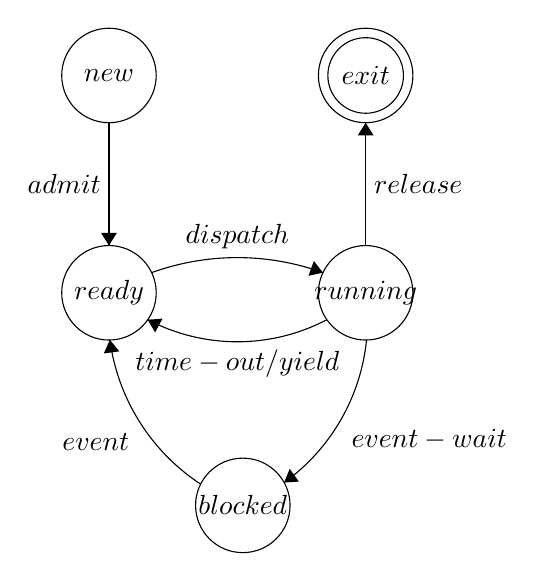
\begin{tikzpicture}[scale=0.2]
    \tikzstyle{every node}+=[inner sep=0pt]
        \draw [black] (22.4,-10.2) circle (3);
        \draw (22.4,-10.2) node {$new$};
        \draw [black] (22.4,-24) circle (3);
        \draw (22.4,-24) node {$ready$};
        \draw [black] (30.9,-37.5) circle (3);
        \draw (30.9,-37.5) node {$blocked$};
        \draw [black] (38.7,-24) circle (3);
        \draw (38.7,-24) node {$running$};
        \draw [black] (38.7,-10.2) circle (3);
        \draw (38.7,-10.2) node {$exit$};
        \draw [black] (38.7,-10.2) circle (2.4);
        \draw [black] (22.4,-13.2) -- (22.4,-21);
        \fill [black] (22.4,-21) -- (22.9,-20.2) -- (21.9,-20.2);
        \draw (21.9,-17.1) node [left] {$admit$};
        \draw [black] (38.7,-21) -- (38.7,-13.2);
        \fill [black] (38.7,-13.2) -- (38.2,-14) -- (39.2,-14);
        \draw (39.2,-17.1) node [right] {$release$};
        \draw [black] (25.109,-22.72) arc (109.90828:70.09172:15.98);
        \fill [black] (35.99,-22.72) -- (35.41,-21.98) -- (35.07,-22.92);
        \draw (30.55,-21.27) node [above] {$dispatch$};
        \draw [black] (36.242,-25.706) arc (-62.26063:-117.73937:12.228);
        \fill [black] (24.86,-25.71) -- (25.33,-26.52) -- (25.8,-25.64);
        \draw (30.55,-27.61) node [below] {$time-out/yield$};
        \draw [black] (28.226,-36.154) arc (-123.29907:-172.30946:13.051);
        \fill [black] (22.46,-26.99) -- (22.07,-27.85) -- (23.06,-27.72);
        \draw (23.72,-33.5) node [left] {$event$};
        \draw [black] (38.755,-26.993) arc (-5.71279:-54.32395:12.711);
        \fill [black] (33.52,-36.05) -- (34.46,-35.99) -- (33.88,-35.18);
        \draw (37.77,-33.32) node [right] {$event-wait$};
    \end{tikzpicture}
\end{center}

\begin{definition}[Context switching]
    \textbf{Context switching} is the process of storing the state of a thread (in a PCB) so that it can be restored and the execution can be resumed at some later point. This is a core idea in process scheduling.
\end{definition}

